\begin{frame}
\frametitle{Electrolysis}
\begin{columns}
    \column[t]{5cm}
	\begin{figure}[htbp!]
		\begin{center}
			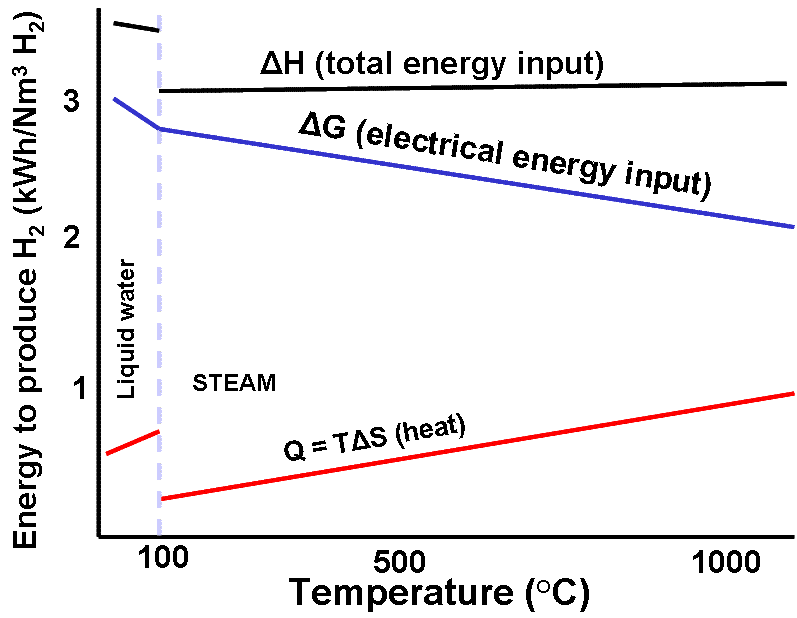
\includegraphics[height=4.0cm]{images/ele-curve.png}
		\end{center}
		\caption{Energy consumption of an ideal electrolysis process \cite{hi2h2_highly_2007}.}
	\end{figure}

	\column[t]{5cm}
	$\Delta$H: Required energy.
	\\
	$\Delta$G: Electrical energy.
	\\
	T$\Delta$S: Thermal energy. \vspace{0.7cm}

    In low temperature electrolysis (LTE), electricity provides the thermal energy.
    \\
    In high temperature electrolysis (HTE), heat source provides the thermal energy.
    \\
    HTE has the advantage of decreasing the electricity requirement.
    
\end{columns}
\end{frame}


\begin{frame}
\frametitle{Sulfur-Iodine}
\begin{columns}
    \column[t]{5cm}
   	\begin{figure}[htbp!]
		\begin{center}
			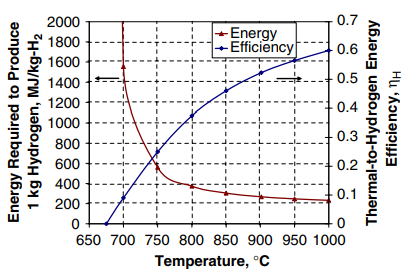
\includegraphics[height=4.0cm]{images/si-energy.png}
		\end{center}
		\caption{Sulfur-Iodine thermochemical cycle.}
 	\end{figure}

 	\column[t]{5cm}
 	\begin{itemize}
 		\item 3 different reactions: Sulfuric acid decomposition, Bunsen reaction, and hydrogen iodide decomposition.
 		\item Input: H$_2$O.
 		\item Output: H$_2$ $\&$ O$_2$. 
 		\item Does not require electricity.
 		\item Need of a high temperature source.
 	\end{itemize}
\end{columns}
\end{frame}


\begin{frame}
\frametitle{Co-generation}
\begin{columns}
    \column[t]{6.5cm}
   	\begin{figure}[htbp!]
		\begin{center}
			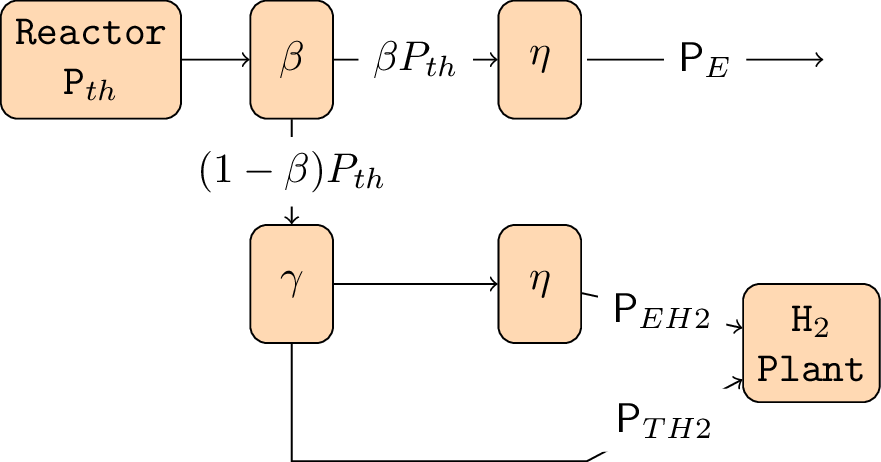
\includegraphics[height=3.6cm]{images/hte-figure0.png}
		\end{center}
		\caption{Reactor coupled to hydrogen plant diagram.}
 	\end{figure}

 	\column[t]{3.5cm}
 	$\beta$: power fraction that is converted into electricity.
 	\\
    $\beta$ = 1: no hydrogen is produced.
    \\
 	$\beta$ = 0: no electricity is produced. \vspace{0.6cm}

 	LTE:
 	\begin{itemize}
 		\item $\gamma$=1. P$_{TH2}$ = 0.
 	\end{itemize}

 	HTE:
 	\begin{itemize}
 		\item 0 $< \gamma <$ 1.
 	\end{itemize}

    SI:
 	\begin{itemize}
 		\item $\gamma$=0. P$_{EH2}$ = 0.
 	\end{itemize}


\end{columns}
\end{frame}